\hypertarget{cv:gestionarActores}{\section{Gestionar Actores}} \label{sec:GestionarActores}

	Esta funcionalidad le permitirá las acciones necesarias para controlar los actores y visualizarlos en una tabla en el proyecto sobre el que se está operando y solicitar el registro de uno nuevo.

		\subsection{Procedimiento}

			%Pasos de procedimiento
			\begin{enumerate}
				
			\item Ingrese a un proyecto existente desde la pantalla \ref{fig:GestionarProyectosColaborador}.
	
			\item Seleccione la opción \textbf{Actores} del menú \ref{fig:MN-LPC}.
	
			\item Se mostrará la pantalla \ref{fig:GestionarActores} ''Gestionar Actores''.

			%Pantalla
			\begin{figure}[h!]
				\begin{center}
					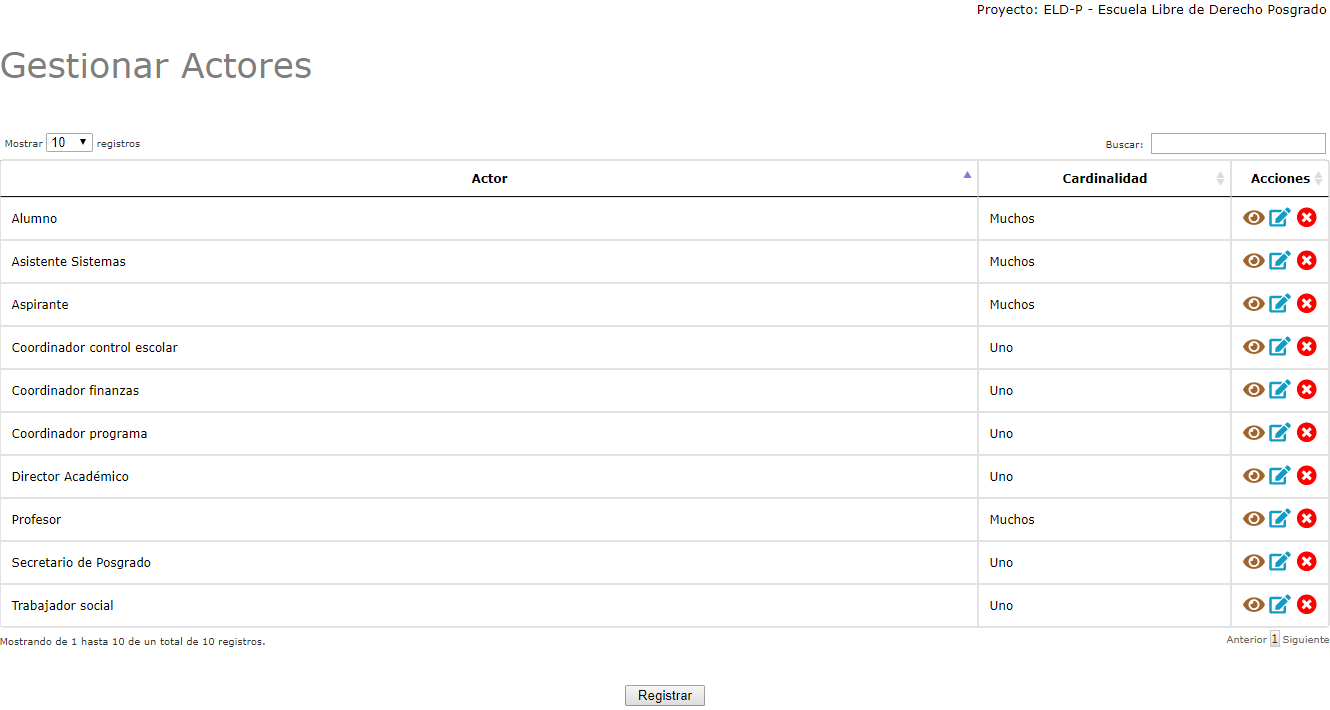
\includegraphics[scale=0.5]{roles/lider/actor/pantallas/IU10gestionarActores}
					\caption{Gestionar Actores}
					\label{fig:GestionarActores}
				\end{center}
			\end{figure}
		
				\item Seleccione la operación que desea realizar:
			
			Para (\hyperlink{cv:registrarActor}{Registrar}) dé clic en el botón \IURegistrar.
			
			Para (\hyperlink{cv:modificarActor}{Modificar}) dé clic en el icono \IUEditar{} de algún actor ya registrado.
			
			Para (\hyperlink{cv:eliminarActor}{Eliminar}) dé clic en el icono \IUBotonEliminar{} de algún actor ya registrado.
			
			Para (\hyperlink{cv:consultarActor}{Consultar}) dé clic en el icono \IUConsultar{} de algún actor ya registrado.
			\end{enumerate}